\begin{figure}[tb]
  \centering
  % \subfloat[]{%
    % 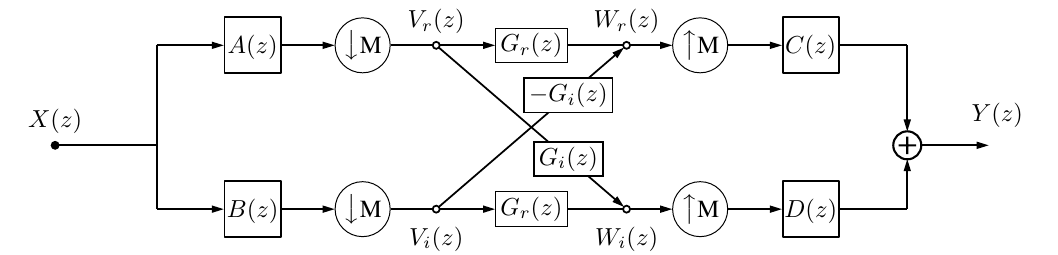
\includegraphics[width=.85\textwidth]{freqlearn/images/top_block.png}
    % \label{fig:ch6:fwd_pass}
  % }
   % \newline
  % \subfloat[]{%
    % 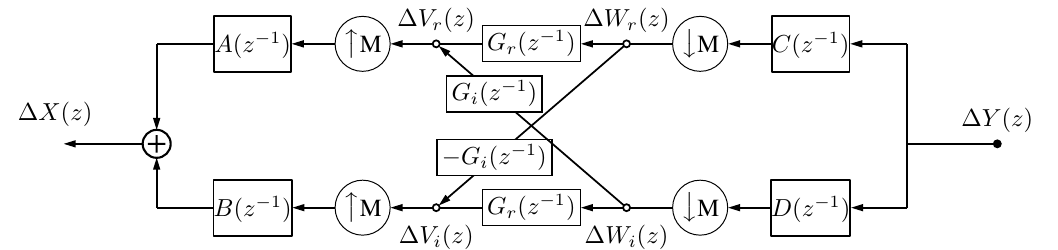
\includegraphics[width=.85\textwidth]{freqlearn/images/bottom_block.png}
    % \label{fig:ch6:bwd_pass}
  % }
  \begin{tikzpicture}
    \matrix (m1) [row sep=5mm, column sep=6mm,align=center,anchor=center]
	{
	% %--------------------------------------------------------------------
		% \node[coordinate]                  (m00) {};    &
		% \node[coordinate]                  (m01) {};          &
		% \node[dspsquare]                   (m02) {$A(z)$};          &
		% \node[circle,draw,inner sep=1pt]   (m03) {\downsamplertext{M}}; &
		% \node[dspnodeopen,dsp/label=above] (m04) {$V_r(z)$};          &
		% \node[rectangle,draw,inner sep=2pt](m05) {$G_r(z)$}; &
		% \node[dspnodeopen,dsp/label=above] (m06) {$W_r(z)$};          &
		% \node[circle,draw,inner sep=1pt]   (m07) {\upsamplertext{M}}; &
		% \node[dspsquare]                   (m08) {$C(z)$};          &
		% \node[coordinate]                  (m09) {};          &
		% \node[coordinate]                  (m0X) {};          \\
		% %--------------------------------------------------------------------
		% \node[]                            (m10) {$X(z)$};          &
		% \node[coordinate]                  (m11) {};          &
		% \node[coordinate]                  (m12) {};    &
		% \node[coordinate]                  (m13) {};          &
		% \node[coordinate]                  (m14) {};    &
		% \node[coordinate]                  (m15) {};          &
		% \node[coordinate]                  (m16) {};    &
		% \node[coordinate]                  (m17) {};          &
		% \node[coordinate]                  (m18) {};    &
		% \node[dspadder]                    (m19) {};          &
    % \node[]                            (m1X) {$Y(z)$};          \\
		% %--------------------------------------------------------------------
		% \node[coordinate]                  (m20) {};    &
		% \node[coordinate]                  (m21) {};          &
		% \node[dspsquare]                   (m22) {$B(z)$};          &
		% \node[circle,draw,inner sep=1pt]   (m23) {\downsamplertext{M}}; &
		% \node[dspnodeopen,dsp/label=below] (m24) {$V_i(z)$};          &
		% \node[rectangle,draw,inner sep=2pt](m25) {$G_r(z)$}; &
		% \node[dspnodeopen,dsp/label=below] (m26) {$W_i(z)$};          &
		% \node[circle,draw,inner sep=1pt]   (m27) {\upsamplertext{M}}; &
		% \node[dspsquare]                   (m28) {$D(z)$};          &
		% \node[coordinate]                  (m29) {};          &
		% \node[coordinate]                  (m2X) {};          \\
		% %--------------------------------------------------------------------
		% &&&&&&&&& \\
		\node[coordinate]                  (m00a) {};    &
		\node[coordinate]                  (m01a) {};          &
		\node[dspsquare]                   (m02a) {$A\left(z^{-1}\right)$};          &
		\node[circle,draw,inner sep=1pt]   (m03a) {\upsamplertext{M}}; &
		\node[dspnodeopen,dsp/label=above] (m04a) {$\Delta U_r(z)$};          &
		%\node[coordinate]                  (m05) {}; &
		\node[rectangle,draw,inner sep=2pt](m05a) {$G_r\left(z^{-1}\right)$}; &
		\node[dspnodeopen,dsp/label=above] (m06a) {$\Delta V_r(z)$};          &
		\node[circle,draw,inner sep=1pt]   (m07a) {\downsamplertext{M}}; &
		\node[dspsquare]                   (m08a) {$C\left(z^{-1}\right)$};          &
		\node[coordinate]                  (m09a) {};          &
		\node[coordinate]                  (m0Xa) {};          \\
		%--------------------------------------------------------------------
		%\node[coordinate]  (m10) {$\Delta X(z)$};          &
    \node[]                            (m10a) {$\Delta X(z)$}; &
		\node[dspadder]                    (m11a) {};          &
		\node[coordinate]                  (m12a) {};    &
		\node[coordinate]                  (m13a) {};          &
		\node[coordinate]                  (m14a) {};    &
		\node[coordinate]                  (m15a) {};          &
		\node[coordinate]                  (m16a) {};    &
		\node[coordinate]                  (m17a) {};          &
		\node[coordinate]                  (m18a) {};    &
		\node[coordinate]                  (m19a) {};          &
		\node[]                            (m1Xa) {$\Delta Y(z)$};          \\
		%--------------------------------------------------------------------
		\node[coordinate]                  (m20a) {};    &
		\node[coordinate]                  (m21a) {};          &
		\node[dspsquare]                   (m22a) {$B\left(z^{-1}\right)$};          &
		\node[circle,draw,inner sep=1pt]   (m23a) {\upsamplertext{M}}; &
		\node[dspnodeopen,dsp/label=below] (m24a) {$\Delta U_i(z)$};          &
		%\node[coordinate]                  (m25) {}; &
		\node[rectangle,draw,inner sep=2pt](m25a) {$G_r\left(z^{-1}\right)$}; &
		\node[dspnodeopen,dsp/label=below] (m26a) {$\Delta V_i(z)$};          &
		\node[circle,draw,inner sep=1pt]   (m27a) {\downsamplertext{M}}; &
		\node[dspsquare]                   (m28a) {$D\left(z^{-1}\right)$};          &
		\node[coordinate]                  (m29a) {};          &
		\node[coordinate]                  (m2Xa) {};          \\
		%--------------------------------------------------------------------
	};
	% \draw[dspline] (m10) -- (m11);
	% \draw[dspline] (m11) -- (m01);
	% \draw[dspline] (m11) -- (m21);
	% \foreach \i in {0,2} {
      % \draw[dspconn] (m\i1) -- (m\i2);
      % \draw[dspconn] (m\i2) -- (m\i3);
      % \draw[dspline] (m\i3) -- (m\i4);
      % \draw[dspconn] (m\i4) -- (m\i5);
      % \draw[dspline] (m\i5) -- (m\i6);
      % \draw[dspconn] (m\i6) -- (m\i7);
      % \draw[dspconn] (m\i7) -- (m\i8);
      % \draw[dspline] (m\i8) -- (m\i9);
	% }
	% %\draw[dspflow] (m04) --  (m06);
	% %\draw[dspflow] (m24) -- (m26);
	% \draw[dspconn] (m24) -- node[draw,pos=0.7,inner sep=2pt,fill=white] {$-G_i(z)$} (m06);
	% \draw[dspconn] (m04) -- node[draw,pos=0.7,inner sep=2pt,fill=white] {$G_i(z)$} (m26);
	% \draw[dspconn] (m09) -- (m19);
	% \draw[dspconn] (m29) -- (m19);
	% \draw[dspconn] (m19) -- (m1X);
	\draw[dspconn] (m11a) -- (m10a);
	\draw[dspconn] (m01a) -- (m11a);
	\draw[dspconn] (m21a) -- (m11a);
	\foreach \i in {0,2} {
    	\draw[dspconn] (m\i9a) -- (m\i8a);
    	\draw[dspconn] (m\i8a) -- (m\i7a);
    	\draw[dspline] (m\i7a) -- (m\i6a);
    	\draw[dspconn] (m\i6a) -- (m\i5a);
    	\draw[dspline] (m\i5a) -- (m\i4a);
    	\draw[dspconn] (m\i4a) -- (m\i3a);
    	\draw[dspconn] (m\i3a) -- (m\i2a);
    	\draw[dspline] (m\i2a) -- (m\i1a);
	}
	%\draw[dspflow] (m04) --  (m06);
	%\draw[dspflow] (m24) -- (m26);
	\draw[dspconn] (m06a) -- node[draw,pos=0.7,inner sep=2pt,fill=white] {$-G_i\left(z^{-1}\right)$} (m24a);
	\draw[dspconn] (m26a) -- node[draw,pos=0.7,inner sep=2pt,fill=white] {$G_i\left(z^{-1}\right)$} (m04a);
	\draw[dspline] (m09a) -- (m19a);
	\draw[dspline] (m29a) -- (m19a);
	\draw[dspline] (m19a) -- (m1Xa);
	
\end{tikzpicture}

  \mycaption{Forward and backward block diagrams for $\DTCWT$ gain layer}{Based
    on Figure~4 in \cite{kingsbury_complex_2001}. Ignoring the $G$ gains, the
    top and bottom paths (through $A, C$ and $B, D$ respectively) make up the
    the real and imaginary parts for \emph{one subband} of the dual tree system.
    Combined, $A+jB$ and $C-jD$ make the complex filters necessary to have
    support on one side of the Fourier domain (see
    \autoref{fig:ch6:dtcwt_bands}). Adding in the complex gain $G_r + jG_i$, we
    can now attenuate/shape the impulse response in each of the subbands. To
    allow for learning, we need backpropagation. The bottom diagram indicates
    how to pass gradients $\Delta Y(z)$ through the layer. Note that upsampling
    has become downsampling, and convolution has become convolution with the
  time reverse of the filter (represented by $z^{-1}$ terms).}
  \label{fig:ch6:fwd_bwd}
\end{figure}


